%
% main.tex -- Paper zum Thema <thema>
%
% (c) 2018 Hochschule Rapperswil
%
\chapter{Achsneigung und Eiszeiten\label{chapter:neigung}}
\lhead{Achseneigung und Eiszeiten}
\begin{refsection}
\chapterauthor{Sebastian Lenhard}

\section{Einführung}\label{sec:einf} \rhead{Einführung}
Das Energie Haushaltsmodell wird verwendet um die Erdtemperatur
theoretisch zu erklären. Dabei wird die Erde als Kugel betrachtet,
die konstant von der Sonne angestrahlt wird. Die eingestrahlte
Energie führt zur Erwärmung der Erde. Die Erde ihrerseits strahlt
ebenfalls Energie ab, wie jedes bestrahlte Objekt. Dabei wird die
Erde als schwarzer Körper modelliert, wodurch die Abstrahlung mit
der Stefan-Bolzmann-Gesetz modelliert werden kann. Die Änderung der
Erdtemperatur kann somit mit der Gleichung
\begin{eqnarray}
\label{eq1}
C \frac{d T}{d t} = (1-\alpha(T)) Q- \varepsilon \sigma T^4
\end{eqnarray}
modelliert werden. Die linke Seite der Gleichung entsprich der
Veränderung der Erdtemperatur, wobei $C$ der Wärmekapazität entspricht,
$T$ die Temperatur in Kelvin und $t$ die Zeit darstellt. Die
Einstrahlung $Q$ wird dabei nicht vollständig von der Erde absorbiert,
ein Teil der Energieeinstrahlung wird reflektiert und hängt von der
Albedo $\alpha(T)$ ab, wobei die Albedo ihrerseits temperaturabhängig
ist. Je kälter die Erde ist, desto höher ist der Albedo der Erde,
da hellere Flächen wie Eis weniger Energie aufnehmen als dunkle
Flächen. Dieser temperaturabhängige Albedo kann durch die Gleichung
\begin{eqnarray} 
\alpha(T) = 0.5 - 0.2 \tanh \left( \frac{T-265}{10} \right) 
\end{eqnarray}
dargestellt werden. Dadurch ist der Albedo symmetrisch um 265 K und
kann maximal zwischen 0.3 und 0.7 schwanken. Die Gleichgewichtstemperatur
ist dabei erreicht, wenn sich die Temperatur über die Zeit nicht
mehr ändert. Abbildung \ref{fig:abb1} zeigt die Einstrahlung und
Ausstrahlung je nach Temperatur. Schnittpunkte sind
Gleichgewichtstemperaturen. Der mittlere Schnittpunkt ist dabei ein
instabiles Gleichgewicht, da mit einer minimal höheren Temperatur
die Einstrahlung höher ist als die Ausstrahlung, wodurch sich die
Erde erwärmt und in das stabile warme (rechte) Gleichgewicht bewegt.
Die selbe Argumentation gilt mit einer minimal tieferen Temperatur,
wodurch die Erde sich auf das kalte (linke) Gleichgewicht zubewegt.
Die ausführliche Herleitung befindet sich in Kapitel 5.
%
%ABBILDUNG1
\begin{figure}
	\centering
	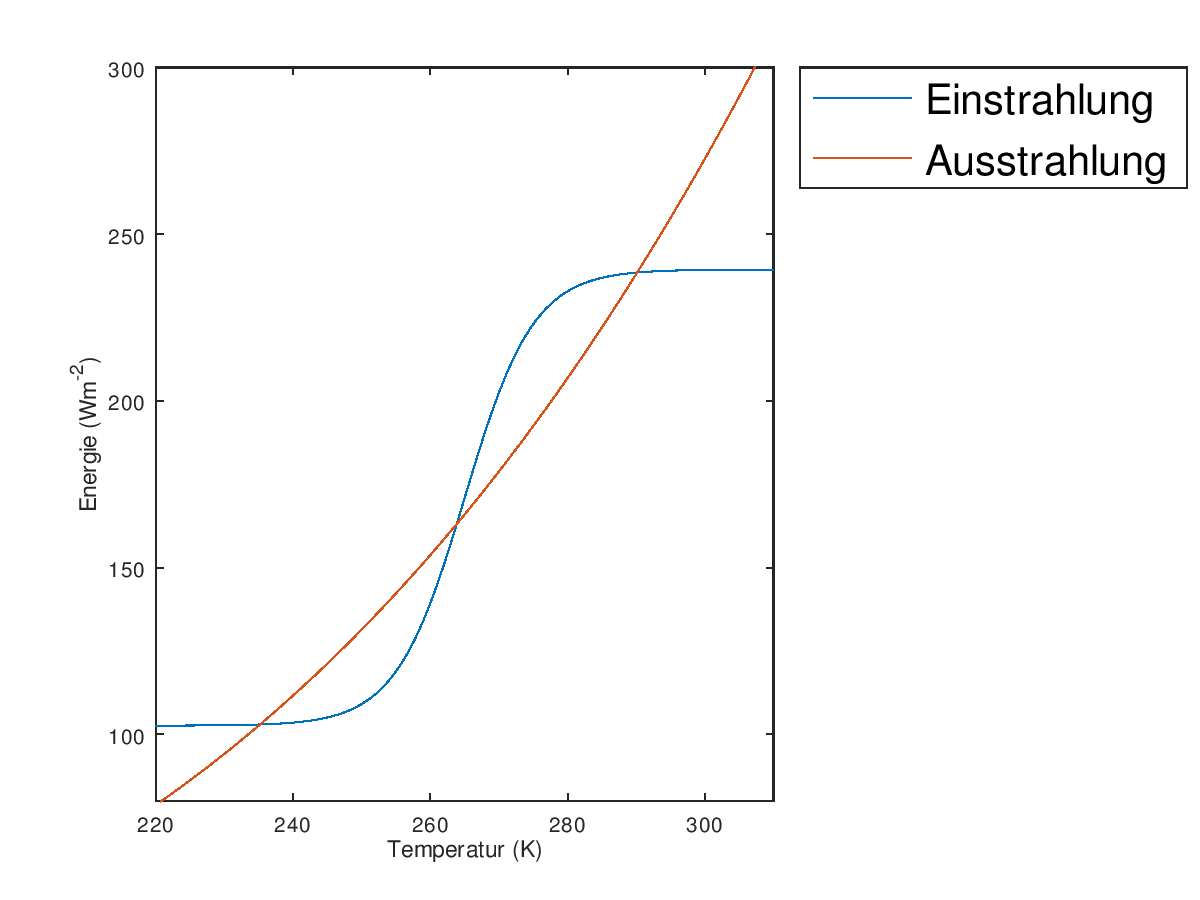
\includegraphics[width= 0.8\textwidth]{neigung/Strahlung_1.png}
	\caption[Gleichgewichtstemperatur]{Gleichgewichtstemperatur}
	\label{fig:abb1}
\end{figure}

Die Neigung der Erdachse bewirkt die Jahreszeiten. Der genaue
\index{Neigung der Erdachse}%
Zusammenhang wird in Abschnitt \ref{sec:winkel} und \ref{sec:neigung}
erläutert. Je grösser der Neigungswinkel, desto extremer sind die
Jahreszeiten. Durch die Jahreszeiten kommt es zu Schwankungen der
Gleichgewichtstemperatur. Dies wird in Abschnitt \ref{sec:bi} anhand
einer Simulation gezeigt. Starke Schwankungen können dazu führen,
dass das Erdklima vom warmen ins kalte Gleichgewicht wechselt und
eine Eiszeit entsteht. Da die Jahreszeiten auf der Nordhalbkugel
und Südhalbkugel jeweils entgegengesetzt zueinander auftreten wird
der Fokus auf eine Halbkugel gelegt (ohne Energieaustausch). In
Abschnitt \ref{sec:math} wird eine Halbkugel mathematisch modelliert
und das Klima wird unter verschiedenen Erdachsenneigungen prognostiziert.
Abschnitt\ref{sec:schluss} fasst die wichtigsten Erkenntnisse
nochmals zusammen und gibt einen Ausblick für weitere Erweiterungen
des Modells.

\subsection{Milankovi\'c Zyklen}\label{sec:mil}
In diesem Abschnitt wird eine kurze empirisch bestätigter Ausblick
über das Verhalten der Erde gegeben. Der serbische Mathematiker
Milutin Milankovi\'c hat Mitte des 20. Jahrhunderts folgende
Entdeckung gemacht: Die Erde bewegt sich in verschiedenen Zyklen
auf ihrer Umlaufbahn.
Zudem führen Störungen durch die grossen Planeten dazu, dass es zu
Schwankungen der Achsenneigung kommen kann. Milakovi\'c unterteilt
die Effekte in drei Zyklen. Die Milankovi\'c Zyklen wurden empirisch
bestätigt.

\subsubsection{Präzession}
Der erste Zyklus wird Präzession genannt und hat eine Länge von
$23\,000$ Jahren. Dieser Zyklus wird durch eine Bewegung der Erdachse
und eine Bewegung der Ellipse der Erdbahn hervorgerufen. Durch die
Anziehungskraft von Sonne und Mond ausgehend, wird die Erdachse
in ein Taumeln gebracht, wie ein aus dem Gleichgewicht geratener
Kreisel. Dagegen wirkt eine zweite Kraft, die durch den Einfluß
aller Planeten unseres Sonnensystems auf die Umlaufbahn der Erde
einfluss nimmt. Beide Bewegungen zusammen bewirken, dass sich die
Jahreszeiten verschieben. Dieser Effekt wird auch als Perihelwanderung
bezeichnet\footnote{Als Perihel wird der Punkt mit dem kleinsten
Abstand auf der Erdumlaufbahn zur Sonne bezeichnet.}.
%
%ABBILDUNG2
\begin{figure}
	\centering
	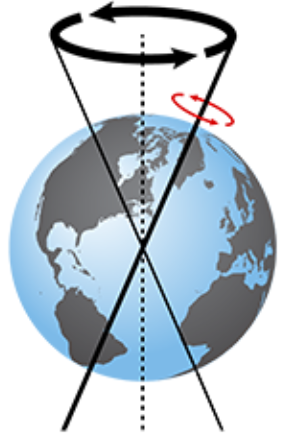
\includegraphics[width= 0.3\textwidth]{neigung/Precession.png}
	\caption[Präzession]{Präzession}
	\label{fig:abb}
\end{figure}

\subsubsection{Exzentrizität}
Der zweite Zyklus ist die Exzentrizität und hat eine Dauer von
100\,000 Jahren. Wie Abbildung \ref{fig:abb2} zeigt, kreist die Erde
um die Sonne. Die Kreisbahn wird allerdings durch den Einfluss der
anderen Planeten verzerrt und zu einer Ellipse geformt. Je nach
Planetenkonstellation ist daher die Umlaufbahn eher kreisförmig oder
nicht. Dieser Effekt ist nur zur Vollständigkeit halber hier
aufgeführt und wird in dem weiteren Verlauf der Arbeit nicht weiter
beachtet. Es wird vereinfacht angenommen, dass die Umlaufbahn der
Erde einem Kreis entspricht.
%
%ABBILDUNG2
\begin{figure}
	\centering
	%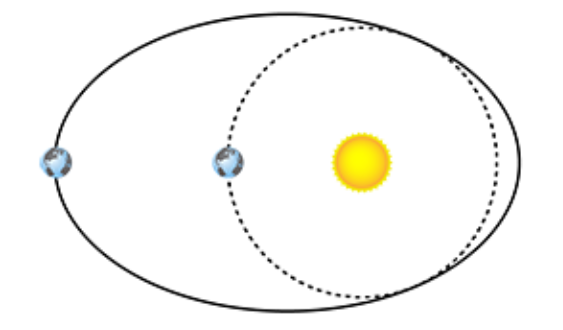
\includegraphics[width= 0.8\textwidth]{neigung/Eccentricity.png}
	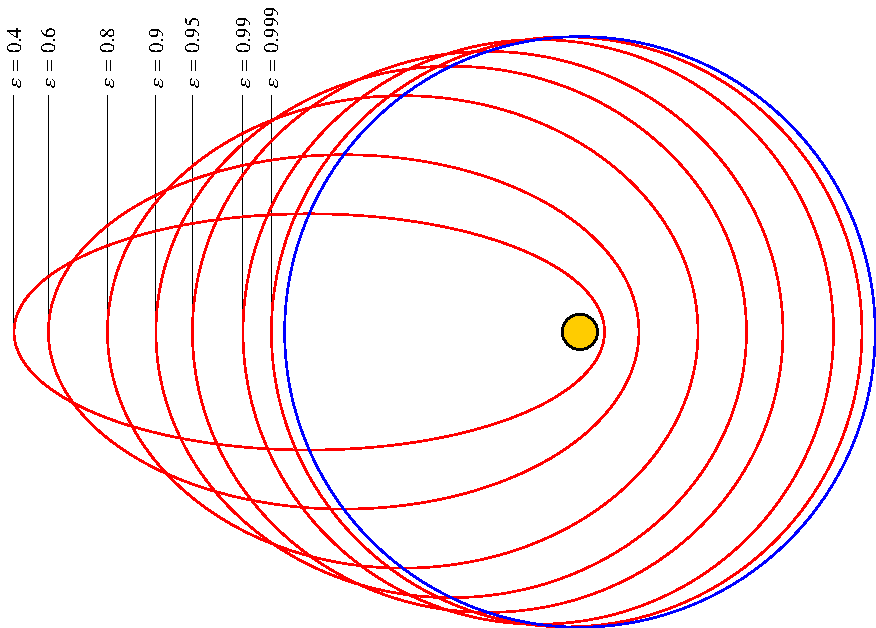
\includegraphics[width= 0.8\textwidth]{neigung/erdbahn.pdf}
	\caption[Exzentrizität]{Exzentrizität}
	\label{fig:abb2}
\end{figure}

\subsubsection{Ekliptikschiefe}
Der letzte Zyklus ist die Ekliptikschiefe und hat einen Rythmus von
41\,000 Jahren. Dabei bewegt sich die Achsenneigung durch den Einfluss
der Planeten. Abbildung \ref{fig:abb3} gibt einen Überblick über
das geschehen. Dieser Zyklus motiviert die folgende Arbeit, die den
Zusammenhang zwischen Klima und dem Winkel der Erdachse untersucht.
Die Abbildungen stammen aus \cite{fm}.
%
%ABBILDUNG3
\begin{figure}
	\centering
	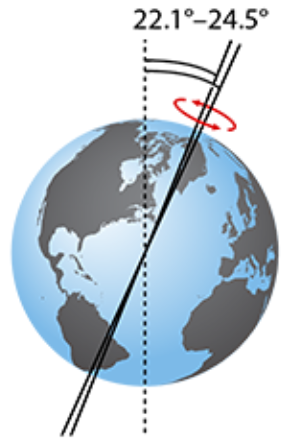
\includegraphics[width= 0.3\textwidth]{neigung/Obliquity.png}
	\caption[Ekliptikschiefe]{Ekliptikschiefe}
	\label{fig:abb3}
\end{figure}
%

\section{Einstrahlungswinkel}\label{sec:winkel}
\rhead{Einstrahlungswinkel}
Da die Erde einen sehr grossen Abstand und nur eine geringe relative
Grösse zur Sonne hat, mit 1:109, wird vereinfacht angenommen, dass
alle Sonnenstrahlen im rechten Winkel auf die Erdkugel treffen.
Nehmen wir zudem vereinfacht an, dass der Neigungswinkel der Erde
$0^\circ$. Dies bedeutet, dass die Sonnenstrahlen am Äquator mit
einem Winkel von $90^\circ$ auf die Erdoberfläche treffen. Durch
die Kugelform der Erde nimmt der Einstrahlungswinkel mit der Distanz
zum Äquator ab. Dies ist in Abbildung \ref{fig:abb5} schematisch
dargestellt.
%
%ABBILDUNG5
\begin{figure}
	\centering
	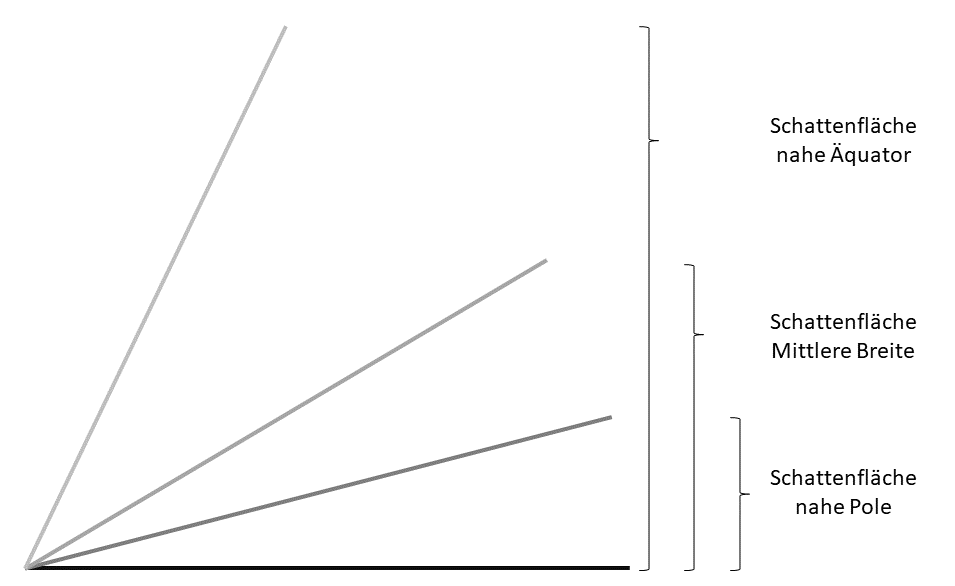
\includegraphics[width= 0.8\textwidth]{neigung/Schatten.png}
	\caption[Einstrahlungswinkel]{Einstrahlungswinkel}
	\label{fig:abb5}
\end{figure}
In der Abbildung kommen die Sonnenstrahlen von der linken Seite.
Beispielsweise ist die angestrahlte Fläche 1$m^2$, zweidimensional
dargestellt als 1$m$ in Abbildung \ref{fig:abb5}. Nahe den Polen
wird die selbe Flächengrösse von weniger Energie bestrahlt, während
am Äquator eine viel grössere Menge an Energie auf die selbe Fläche
trifft. Die eingestrahlte Energiemenge kann als Schattenfläche
aufgefasst werden. In Abbildung \ref{fig:abb5} ist ersichtlich,
dass die Energiemenge pro Fläche am Äquator deshlab erheblich grösser
ist als an den Polen. Der Einstrahlungswinkel beeinflusst somit,
wieviel Energie auftrifft und somit aufgenommen wird. Daraus folgt,
dass es am Äquator wärmer ist als an den Polen.

In diesem Gedankenexperiment wird somit der Äquator konstant in
einem Winkel von $90^\circ$ bestrahlt, während die Pole keine direkte
Strahlung empfangen. Im Verlaufe eines Jahres legt die Erde eine
Umkreisung der Sonne zurück. Vereinfacht wird eine Kreisbahn
angenommen. Mit einem Neigungswinkel von $0^\circ$ ist die Einstrahlung
entlang der Umlaufbahn konstant für jeden Punkt auf der Erde. Im
folgenden Abschnitt wird die Annahme des Neigungswinkel mit $0^\circ$
gelockert und erläutert wie dadurch die Jahreszeiten entstehen.

\section{Achsenneigung}\label{sec:neigung}
\rhead{Achsenneigung}
Durch die Neigung der Erdachse kommt es zu der Entstehung der Jahreszeiten. Dies wird anhand der Abbildung \ref{fig:abb6} intuitiv erklärt. 
%
%ABBILDUNG6
\begin{figure}
	\centering
	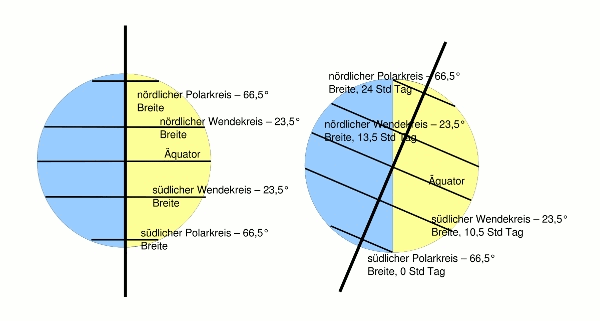
\includegraphics[width= 0.8\textwidth]{neigung/tagundnacht.png}
	\caption[Achsenneigung]{Achsenneigung}
	\label{fig:abb6}
\end{figure}
%
Die linke Erdkugel in Abbildung \ref{fig:abb6} zeigt die Situation
mit einem Neigungswinkel von $0^\circ$. Die Mittlere Linie entspricht
der Breitengrade des Äquators. Wie in Abschnitt \ref{sec:winkel}
erläutert ist somit die Einstrahlung am grössten am Äquator, da die
Sonnenstrahlen in einem Winkel von $90^\circ$ auf die Erdoberfläche
auftreffen. Die rechte Erdkugel illustriert nun einen Neigungswinkel.
Dadurch wird ersichtlich, dass der Äquator nicht länger der Breitengrad
ist, in dem die Sonnenstrahlen in einem Winkel von $90^\circ$
eintreffen. In der Abbildung \ref{fig:abb6} entspricht dies nun der
Linie des Wendekreises. In der Abbildung kommen die Sonnenstrahlen
von der rechten Seite, somit entsprich die gelbe Fläche der
angestrahlten Fläche der Erdkugel. Es ist ersichtlich, dass am
Nordpol dadurch Sonnenstrahlen ankommen, während der Südpol nicht
bestrahlt wird. Im Verlaufe eines Tages dreht sich die Erde einmal
um die eigene Achse. In der rechten Abbildung bedeutet das, dass
am Nordpol keine Nacht stattfindet, während am Südpol ewige Nacht
herrscht. Am Äquator dauert ein Tag genau 12 Stunden, während auf
der Nordhalbkugel die Tage länger sind als auf der Südhalbkugel.
Dies entsprich der Situation Sommer auf der Nordhalbkugel, respektive
Winter auf der Südhalbkugel. Die Abbildung stammt aus \cite{fa}.

Auf ihrer Umlaufbahn um die Sonne bleibt die Erdachse konstant
geneigt. Dies bedeutet, dass im Nordwinter, die Situation entsteht,
in der in Abbildung \ref{fig:abb6} die gelbe Fläche bestrahlt wird
während die blaue Fläche nicht bestrahlt wird. Somit am Nordpol
ewige Nacht herrscht und am Südpol die Sonne nie untergeht. Im
Frühling und im Herbst ist die Strahlungssituation in der linken
Seite abgebildet. Diese kontinuierlichen Übergänge von heissem
Sommer zu kaltem Winter werden im nächsten Abschnitt \ref{sec:math}
mathematisch modelliert. Dabei wird der Fokus auf eine Halbkugel
gelegt, da die Jahreszeiten halbkugelspezifisch auftreten.

\section{Mathematischer Zusammenhang}\label{sec:math}
\rhead{Mathematischer Zusammenhang}
Motiviert durch die vorhergegangenen zwei Abschnitte wird das
Energiehaushaltsmodell aus Abschnitt \ref{sec:einf} erweitert. Im
folgenden wird zuerst in Abschnitt \ref{sec:einst} erläutert, wie
die zyklisch ändernde Einstrahlung mathematisch modelliert wird,
abhängig von der Achsenneigung. In Abschnitt \ref{sec:bi} werden
die Gleichgewichte als Bifurkation zusammengefasst. Abschnitt
\ref{sec:sim1} wird eine Simulation gerechnet und präsentiert. Da
die Simulation zeigt, dass dadurch keine Eiszeit entstehen kann,
wird in Abschnitt \ref{sec:co} die Coalbedo nicht linear transformiert.
Die Simulation wird mit verändertet Coalbedo nochmals gerechnet in
Abschnitt \ref{sim2}. Dadurch wird gezeigt, dass es zu einer Eiszeit
kommen kann.


\subsection{Einstrahlung} \label{sec:einst}
Die Einstrahlung auf eine Halbkugel schwankt zyklisch im Rhythmus
eines Jahres. Anstelle der konstanten Einstrahlung $Q$ im Energie
Haushaltsmodell in Abschnitt \ref{sec:einf} wird nun eine zeitabhängige
Einstrahlung modelliert. Gegeben der Neigungswinkel
$\omega$ Schwankt die Einstrahlung um die Solarkonstante $Q$. $t$
ist die Zeit, die anhand des $\sin(.)$ die Umlaufbahn als Kreisbahn
der Erde um die Sonne modelliert. Je grösser der Neigungswinkel
$\omega$, desto extremer sind die Schwankungen. Dies wird Anhand
der Funktion
\begin{eqnarray*} 
I(t, \omega) = Q+\frac{\sin(\omega)\sin(t)}{\sqrt{1+(\sin(\omega) \sin(t))^2}}Q
\end{eqnarray*}
ermöglicht.  Mit einem Neigungswinkel von $\omega=0$ entspricht das
Modell wieder dem ursprünglichen Energie Haushaltsmodell. Somit
wird die Gleichung \eqref{eq1} modifiziert zu:
\begin{eqnarray} \label{eq2}
C \frac{d T}{d t} = (1-\alpha(T)) I(t, \omega) - \varepsilon \sigma T^4
\end{eqnarray}
Anstelle der Solarkonstanten $Q$ steht in Gleichung \eqref{eq2}
nun die Zeit und winkelabhängige Einstrahlung $I(t,\omega)$. Dadurch
entstehen verschieden Gleichgewichte, die vom jeweiligen Zeitpunkt
und gegeben dem Winkel abhängen. Im Sommer hat die Funktion
$I(t,\omega)$ ein Maximum gegeben $\omega$, während im Winter jeweils
ein Minimum erreicht ist. Die verschiedenen Einstrahlungen sind in
Abbildung \ref{fig:abb7} dargestellt.
%
%ABBILDUNG7
\begin{figure}
	\centering
	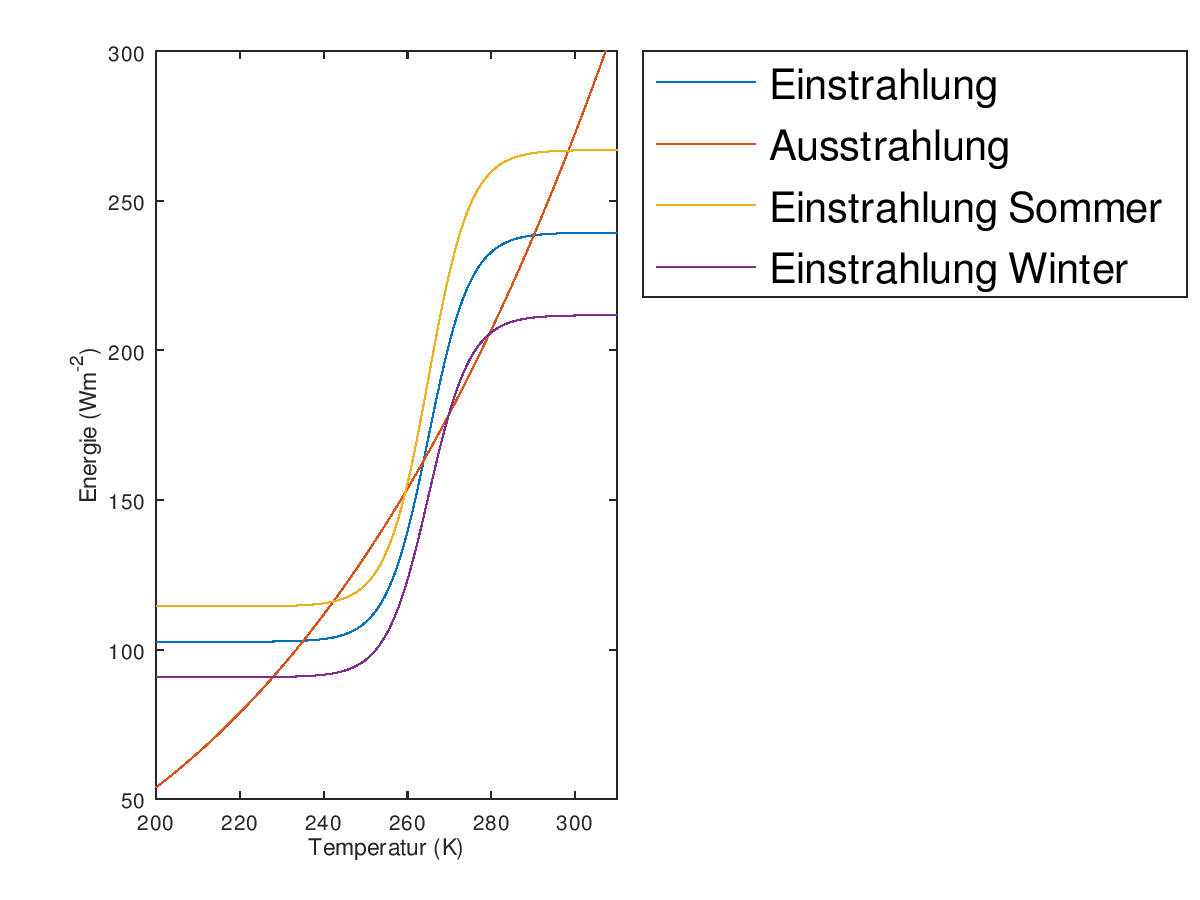
\includegraphics[width= 0.8\textwidth]{neigung/Strahlung_2.png}
	\caption[Gleichgewichtstemperatur]{Gleichgewichtstemperatur}
	\label{fig:abb7}
\end{figure}
Durch die Neigung und die mit ihr einherkommende zyklische Schwankung
der Einstrahlung entstehen somit verschieden Gleichgewichte. Über
ein Jahr bewegt sich die Einstrahlungsfunktion von der violetten
(Winter) Linie kontinuierlich über die blaue (Frühling) zur gelben
(Sommer) und wieder über die blaue (Herbst) zurück. Eine Möglichkeit
dies in einem übersichtlicheren Format darzustellen bietet die
Bifurkation. Diese wird im nächsten Abschnitt \ref{sec:bi} erläutert.


\subsection{Mögliche Eiszeit} \label{sec:bi}
Die Bifurkation zeigt wie sich die Lösungen einer Differentialgleichung
verändern, gegeben die Änderung eines Parameters. Die betrachtete
Differenzialgleichung \eqref{eq1} aus dem ursprünglichen Energie
Haushaltsmodell, indem nun die Einstrahlung $Q$ verändert wird.
Dies ist äquivalent zur Differenzialgleichung \eqref{eq2}.
%
%ABBILDUNG8
\begin{figure}
	\centering
	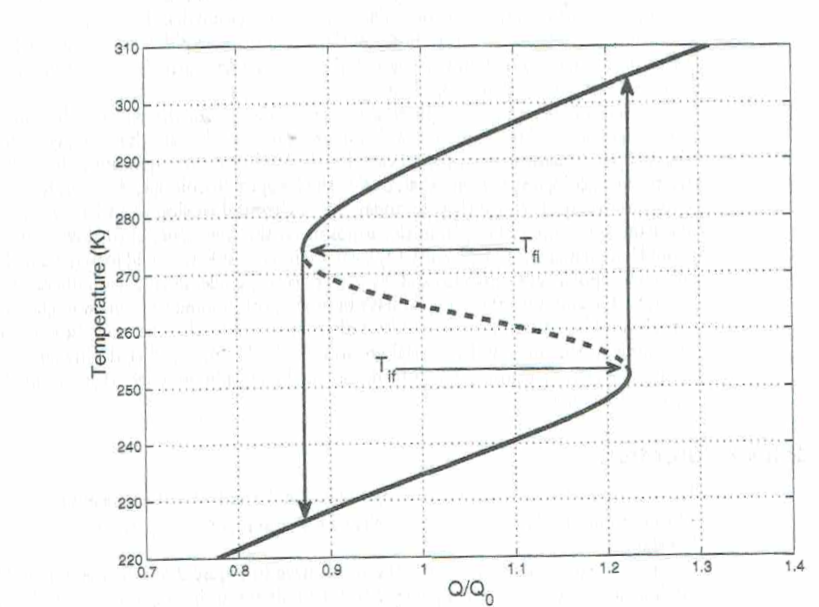
\includegraphics[width= 0.8\textwidth]{neigung/Bifurkation.png}
	\caption[Bifurkation]{Bifurkation}
	\label{fig:abb8}
\end{figure}
%
Betrachtete man in Abbildung \ref{fig:abb7} das warme Gleichgewicht
im Winter und erhöht die Strahlung, so erhöht sich die
Gleichgewichtstemperatur. Dies entsprich in Abbildung \ref{fig:abb8}
der ausgezogenen Linie im oberen Drittel, die einen positiven
Zusammenhang zwischen Einstrahlungsintensität und Gleichgewichtstemperatur
aufweist. Senkt man die Einstrahlung, so ist in Abbildung \ref{fig:abb7}
zu erkennen, dass das warme Gleichgewicht und das instabile
Gleichgewicht auf den selben Punkt fallen indem sich Einstrahlung
und Ausstrahlung tangieren. Dies entspricht in Abbildung \ref{fig:abb8}
dem Zusammentreffen mit der gestrichelten Linie ($T_{fl}$). Eine
weitere Minderung der Einstrahlung hat zur folge, dass das warme
Gleichgewicht nicht mehr existiert, sondern nur noch das kalte
Gleichgewicht.

Die gestrichelte Linie entspricht dem instabilen Gleichgewicht in
Abbildung \ref{fig:abb7}, welches einen negativen Zusammenhang
zwischen Einstrahlung und Gleichgewichtstemperatur hat. In dem Punkt
$T_{lf}$, wo sich das instabile und kalte Gleichgewicht treffen,
ist in Abbildung \ref{fig:abb7} der Fall, wenn die Einstrahlung so
hoch ist, dass das kalte Gleichgewicht mit dem instabilen Gleichgewicht
zusammefällt im Punkt wo sich Einstrahlung und Ausstrahlung tangieren.
Eine weitere Erhöhung der Einstrahlung führt dazu, dass das kalte
Gleichgewicht nicht mehr existiert.

Wie die Bifurkation zeigt, existieren für gewisse Einstrahlungen
drei Gleichgewichte (warmes, instabiles und kaltes) wie in Abbildung
\ref{fig:abb7} dargestelt. Für extrem hohe Einstrahlungen exitiert
lediglich das warme Gleichgewicht während für tiefere Einstrahlungen
lediglich das kalte Gleichgewicht existiert. Die Erde befindet sich
momentan in ihrem warmen Gleichgewicht. Durch die zyklische
Einstrahlung schwankt die Gleichgewichtstemperatur in der oberen
ausgezogenen Linie in Abbildung \ref{fig:abb8}. Durch einen extrem
kalten Winter beziehungsweise durch eine tiefe Einstrahlung kann
es sein, dass die Erde in das kalte Gleichgewicht fällt. Dadurch
würde sie in Zukunft auf der unteren ausgezognen Linie schwanken.
Um eine solche Situation genauer zu untersuchen wird im nächsten
Abschnitt eine Simulation berechnet.


\subsection{Simulation I} \label{sec:sim1}
Durch die Änderung des Neigungswinkels gemäss den Milankovi\'c
Zyklen kann es zu einer möglichen Eiszeit kommen. Dies wird im
Folgenden anhand einer Simulation versucht darzustellen. Dabei wird
die Differenzialgleichung \eqref{eq2} gelöst. Es werden verschiedene
Neigungswinkel $\omega$ verwendet und die Gleichgewichtstemperatur
über die Zeit projizieren. Abbildung \ref{fig:abb9} zeigt das
Ergebnis der Simulationen.
%
%ABBILDUNG9
\begin{figure}
	\centering
	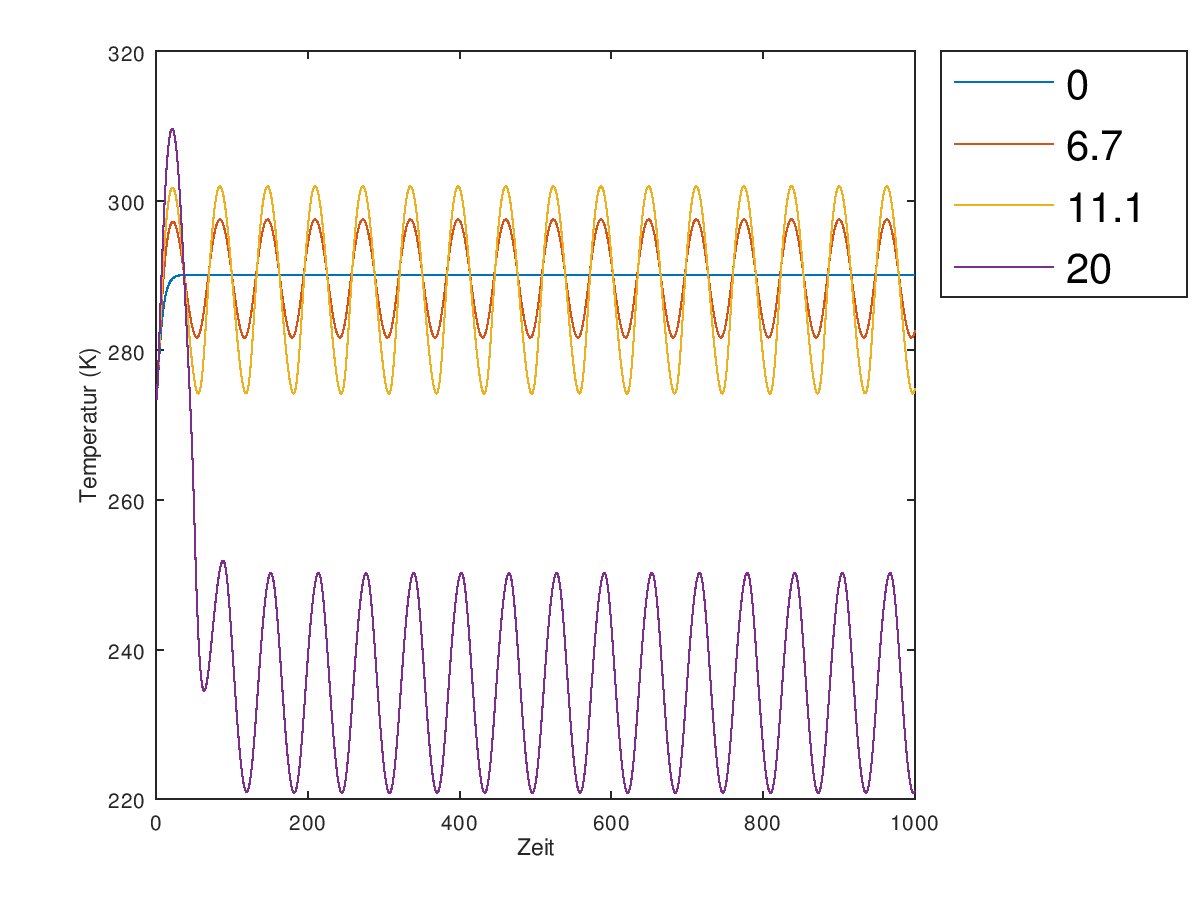
\includegraphics[width= 0.8\textwidth]{neigung/Zeitachse_0.png}
	\caption[Simulation I]{Simulation I}
	\label{fig:abb9}
\end{figure}
%
Als blaue Linie ist dargestellt wie das ursprüngliche
Energiehaushaltsmodell aus Abschnitt \ref{sec:einf} mit einem
Neigungswinkel $\omega=0$ aussieht. Da bei ist ersichtlich, dass
das System unterhalb der Gleichgewichtstemperatur startet und nach
dem ersten Sommer das konstante Gleichgewicht erreicht. In Orange
und Gelb ist ein grösserer Neigungswinkel simuliert. Es ist
ersichtlich, dass das System im warmen Gleichgewicht bleibt und um
dieses herum schwankt. Im violetten Fall ist der Neigungswinkel noch
grösser, was dazu führt , dass das System im ersten Winter sofort
in das kalte Gleichgewicht wechselt und dann in dem kalten Gleichgewicht
schwankt, wie erklärt in Abschnitt \ref{sec:bi}. Die Erde wechselt
von dem warmen in das kalte Gleichgewicht, es bildet sich eine
Eiszeit in der es weiterhin Sommer und Winter gibt, jedoch um ca.
$60 ^\circ$ Kelvin tiefer.

In allen Situationen entscheidet sich das Gleichgewicht bereits
nach der ersten Periode, beziehungsweise im ersten Jahr. In keinem
der Fälle wird sich durch einen längeren Zeitraum ein weiterer
Gleichgewichtswechsel stattfinden. Um eine Transformation zum kalten
Gleichgewicht zu modellieren muss die Albedo beziehungsweise Coalbedo
angepasst werden.


\subsection{Coalbedo} \label{sec:co}
Die temperaturabhängige Albedo ist in Gleichung \eqref{eq2} gegeben
und gibt an wieviel Energie reflektiert wird. Diese ist symmetrisch
um $265\,\text{K}$ und beschränkt zwischen $0.3$ und $0.7$ und reagiert
gleichermassen auf Temperaturerhöhungen wie auf Senkungen. Tiefere
Temperaturen führen zu einer erhöhten Energiereflexion, da sich
grössere Eisflächen bilden und diese die Sonnenstrahlen stärker
reflektieren als die braune oder grüne Erde. Die Coalbedo entspricht
dem Wert $1-\alpha(T)$ und gibt an wieviel Energie von dem Planeten
aufgenommen wird. Mit der Funktion in Gleichung \ref{eq4} wird die
Coalbedo asymmetrisch transformiert.
\begin{eqnarray} \label{eq4}
g(x)=x-a(x-\frac{1}{2})^2
\end{eqnarray}
Input $x$ in der Funktion ist die ursprüngliche symmetrische Coalbedo
$1-\alpha(T)$. In Abbildung \ref{fig:abb10} ist die Transofmationsfunktion
für verschiedene Parameter $a$ dargestellt. Mit $a=0$ bleibt der
lineare Zusammenhang bestehen, während $a>0$ nun asymmetrische
Transformationen erlaubt. Die Transformation führt zu einer tieferen
Coalbedo für hohe beziehungweise tiefe Temperaturen. Bei einer
Temperatur von $265 K$ ist die Coalbedo wiederum $0.5$, wie im
ursprünglichen Modell. Dies bedeutet, dass die Coalbedo stärker
reagiert für tiefere Temperaturen während die Reaktion bei höheren
Temperaturen verlangsamt wird. Dies kann motiviert werden durch das
selbe Argument wie zu Beginn des Abschnittes. Das Eis reflektiert
die Sonnenstrahlen stärker als die brauen oder grüne Erde. Ist das
Eis jedoch geschmolzen, so ist der Effekt einer weiteren
Temperaturerhöhung geringer als der Effekt vor der Eisschmelze.
%
%ABBILDUNG10
\begin{figure}
	\centering
	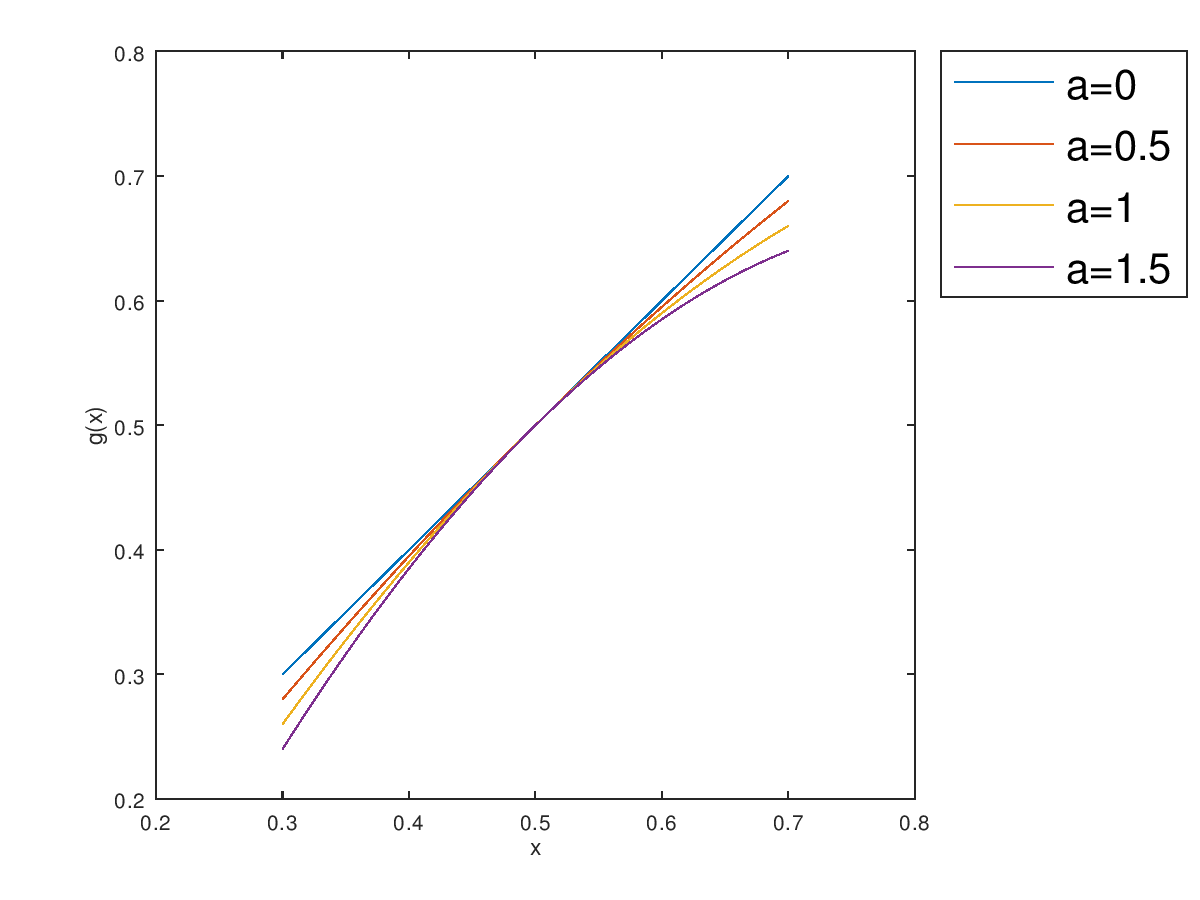
\includegraphics[width= 0.8\textwidth]{neigung/Funktion.png}
	\caption[Asymmetrie in der Coalbedo]{Asymmetrie in der Coalbedo}
	\label{fig:abb10}
\end{figure}
%
Durch diese Transformation wird die Coalbedo zu:
\begin{eqnarray*}
\kappa(T)=(1-\alpha(T)) - a \left( 1-\alpha(T) - \frac{1}{2} \right)^2.
\end{eqnarray*}
Diese hängt wiederum von der Temperatur $T$ ab, ist nun aber
asymmetrisch durch den Parameter $a$ verzerrt. Das Energie
Haushaltsmodell kann nun mit dieser Funktion der Coalbedo erweitert
werden. Somit wird das Modell aus Gleichung \ref{eq2} durch die
folgende Differentialgleichung beschrieben.
\begin{eqnarray} \label{eq5}
C \frac{d T}{d t} =  \kappa(T) I(t, \omega) - \varepsilon \sigma T^4
\end{eqnarray}
Wiederum wird die Gleichgewichtstemperatur ermittelt indem sich die
Temperatur über die Zeit für die gegebenen Parameter nicht ändert
$\frac{d T}{d t}=0$, beziehungsweise die Energie Einstrahlung der
Ausstrahlung der Erde entspricht. Abbildung \ref{fig:abb11} zeigt
die Einstrahlung abhängig von der Temperatur, sowie die Ausstrahlung
abhängig von der Temperatur. Diese Abbildung kann mit Abbildung
\ref{fig:abb7} verglichen werden. Die Ausstrahlung bleibt die selbe,
weiterhin als schwarze Kugel mit dem Stefan-Boltzmann-Gesetz
modelliert. Die Einstrahlung hat sich nun verändert, und ist nun
geringer für Temperaturen $T \neq 265 K$ verglichen mit Abbildung
\ref{fig:abb7}. Dies als Resultat der Transformation der Coalbedo,
da diese für $a>0$ tiefer ist, wie im obigen Abschnitt erklärt. Die
zugehörige Bifurkation sieht schematisch gleich aus wie in Abbildung
\ref{fig:abb8} beschrieben.
%
%ABBILDUNG11
\begin{figure}
	\centering
	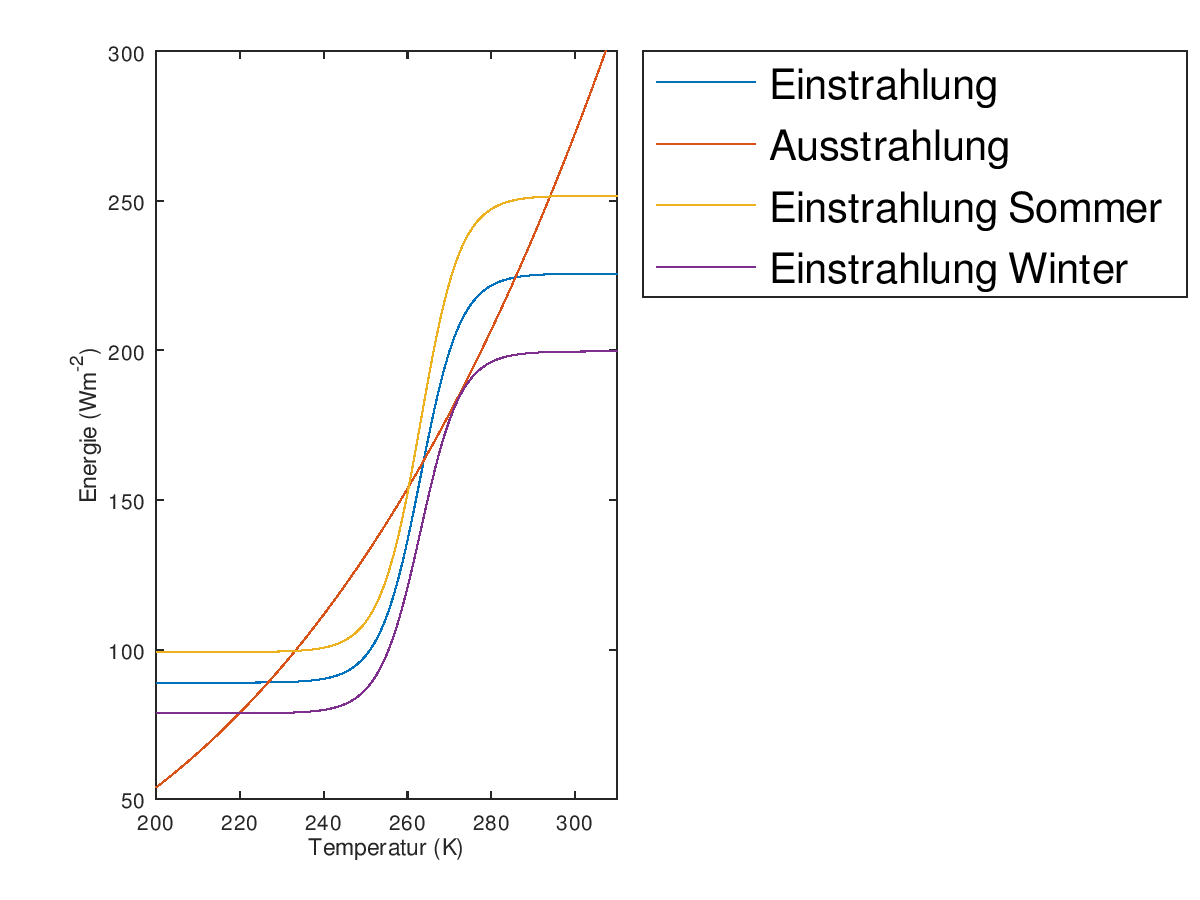
\includegraphics[width= 0.8\textwidth]{neigung/Strahlung_3.png}
	\caption[Gleichgewichtstemperatur]{Gleichgewichtstemperatur}
	\label{fig:abb11}
\end{figure}
%

\subsection{Simulation II} \label{sim2}
In diesem Abschnitt wird erneut eine Simulation gerechnet, welche
nun im Vergleich zu Abschnitt \ref{sec:sim1} die asymmetrische
Coalbedo verwendet. Wiederum werden vier verschiedene Neigungswinkel
simuliert. Zudem werden drei verschiedene Werte für den Parameter
$a$, welcher die Stärke der Asymmetrie bestimmt angenommen. Die
Resultate sind in Abbildung \ref{fig:abb12}--\ref{fig:abb14} dargestellt
und können mit Abbildung \ref{fig:abb9} verglichen werden. In
Abbildung \ref{fig:abb9} ist der Parameter $a=0$, während er für
die restlichen Abbildungen jeweils erhöht wird. In allen drei
folgenden Abbildungen wird klar, dass nun ein Sprung in das kalte
Gleichgewicht möglich ist über die Zeit.
%
%ABBILDUNG12
\begin{figure}
	\centering
	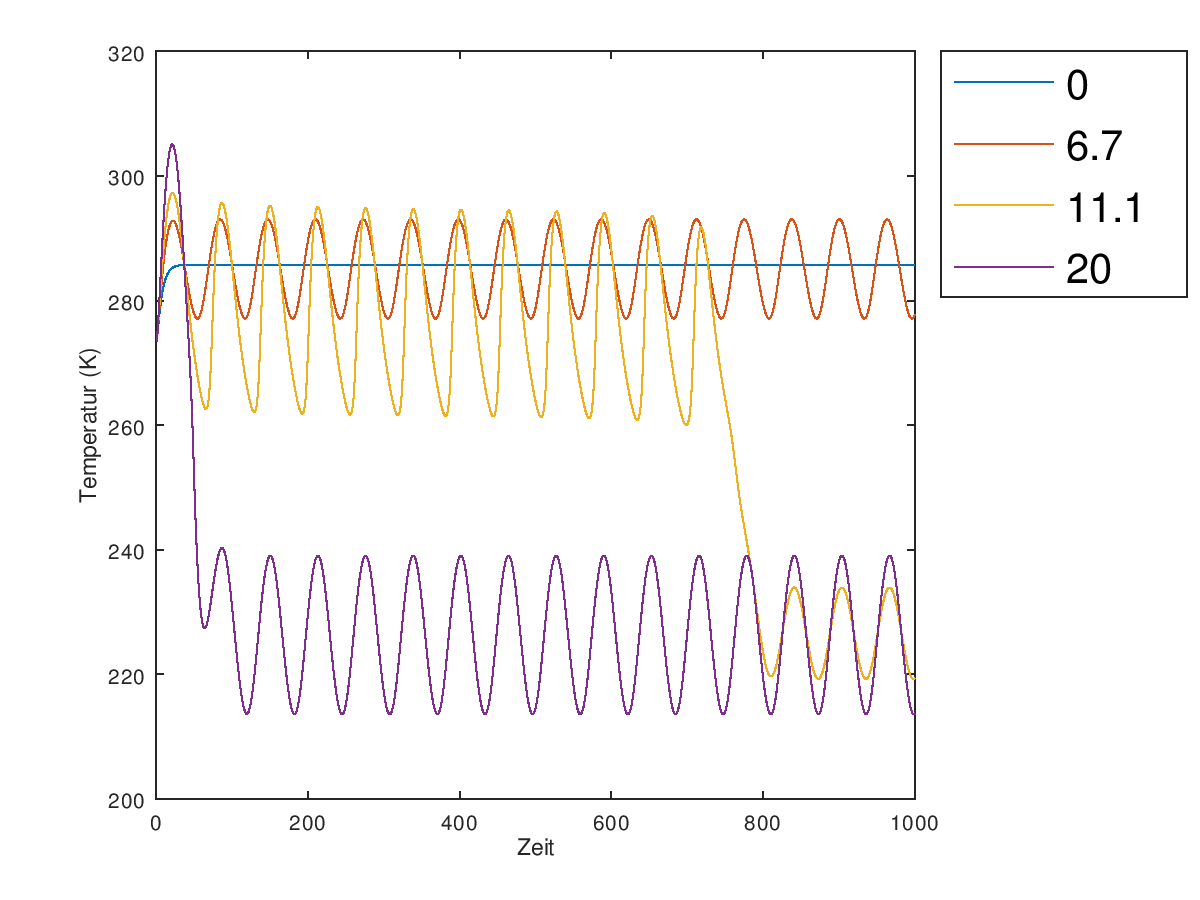
\includegraphics[width= 0.8\textwidth]{neigung/Zeitachse_1.png}
	\caption[Simulation II a]{Simulation II a}
	\label{fig:abb12}
\end{figure}
%
Als blaue Linie ist wiederum der ursprüngliche Fall mit einem
Neigungswinkel von $\omega=0$ dargestellt. Da zu Beginn der Simulation
die Gleichgewichtstemperatur noch nicht erreicht ist, erwärmt sich
die Erde und bleibt konstant im warmen Gleichgewicht. Durch die
Achsenneigung kommt es in dem orangen Fall zu zyklischer Einstrahlung
und somit zu einer schwankenden Temperatur. Die Temperaturschwankung
ist allerdings zu gering, als das ein Sprung in das kalte Gleichgewicht
stattfinden könnte.

Im gelben Fall ist der Neigungswinkel höher als im orangen Fall.
Es kommt zu stärkeren Schwankungen wobei ersichtlich ist, dass diese
asymmetrische nach untern ausreissen. Es wird kälter über die  Zeit,
jeweils im Sommer wie auch im Winter. Bis zum Moment, indem ein
solch kalter Winter erreicht ist, indem das warme Gleichgewicht
nicht mehr existiert, somit findet ein Sprung in das kalte Gleichgewicht
statt. Es ist ebenfalls erkennbar, dass die Schwankungen im kalten
Gleichgewicht geringe ausfallen als im warmen. Dies kommt durch die
Asymmetrie in der Coalbedo.

Im violetten Fall ist die Achsenneigung so gross, dass bereits der
erste Winter so kalt ist, dass die Erde ins kalte Gleichgewicht
wechselt. Es ist auch gut zu erkennen, dass die Schwankungen stärker
sind als in dem gelben Fall im kalten Gleichgewicht. Dies aufgrund
der stärkeren Achsenneigung, die extremere Jahreszeiten zu folge
hat.

In Abbildung \ref{fig:abb13} und \ref{fig:abb14} ist ersichtlich,
wie eine stärkere Asymmetrie in der Coalbedo den Effekt der
Temperatursenkung verstärkt und somit schneller eine Eiszeit erreicht
wird. Dabei gelten die gleichen Effekte wie im obigen Abschnitt
beschrieben.
%
%ABBILDUNG13
\begin{figure}
	\centering
	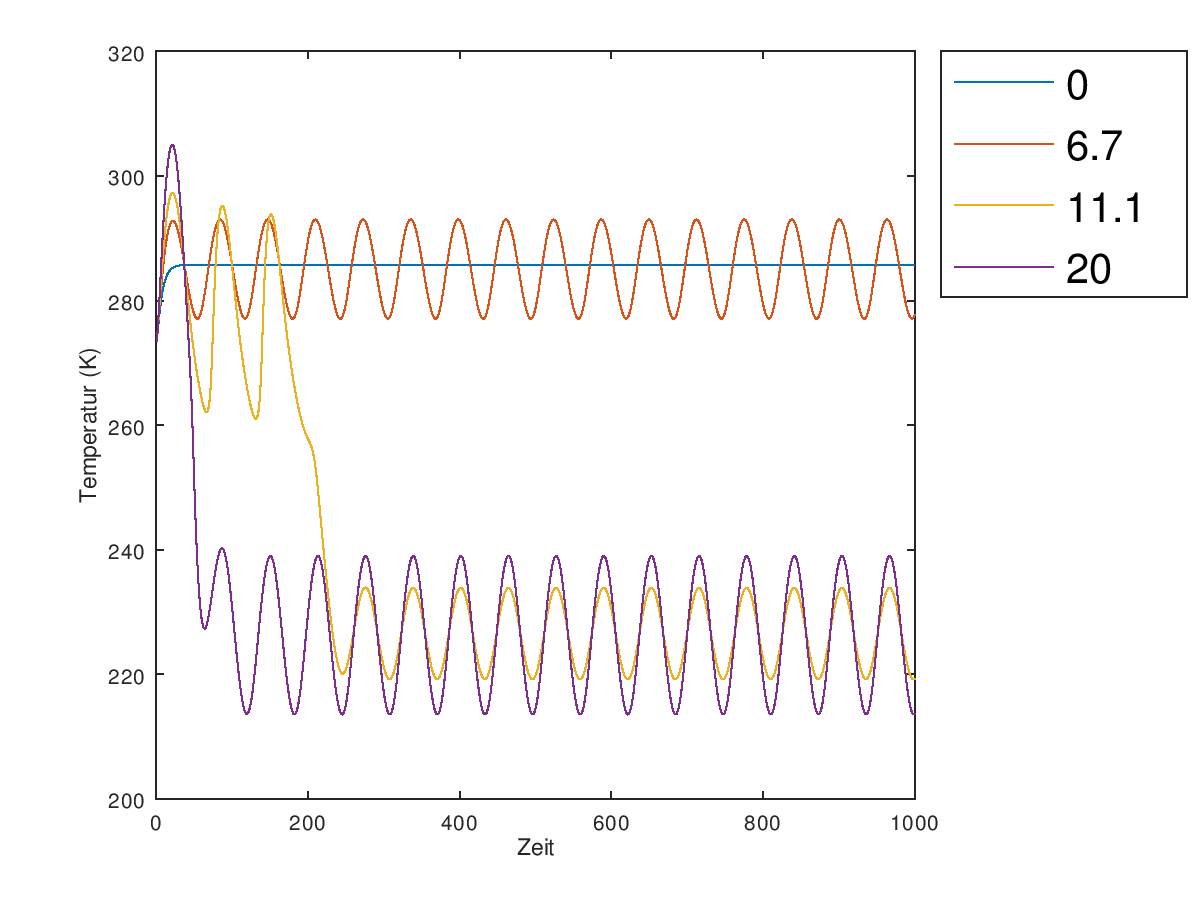
\includegraphics[width= 0.8\textwidth]{neigung/Zeitachse_2.png}
	\caption[Simulation II b]{Simulation II b}
	\label{fig:abb13}
\end{figure}
%
%
%ABBILDUNG14
\begin{figure}
	\centering
	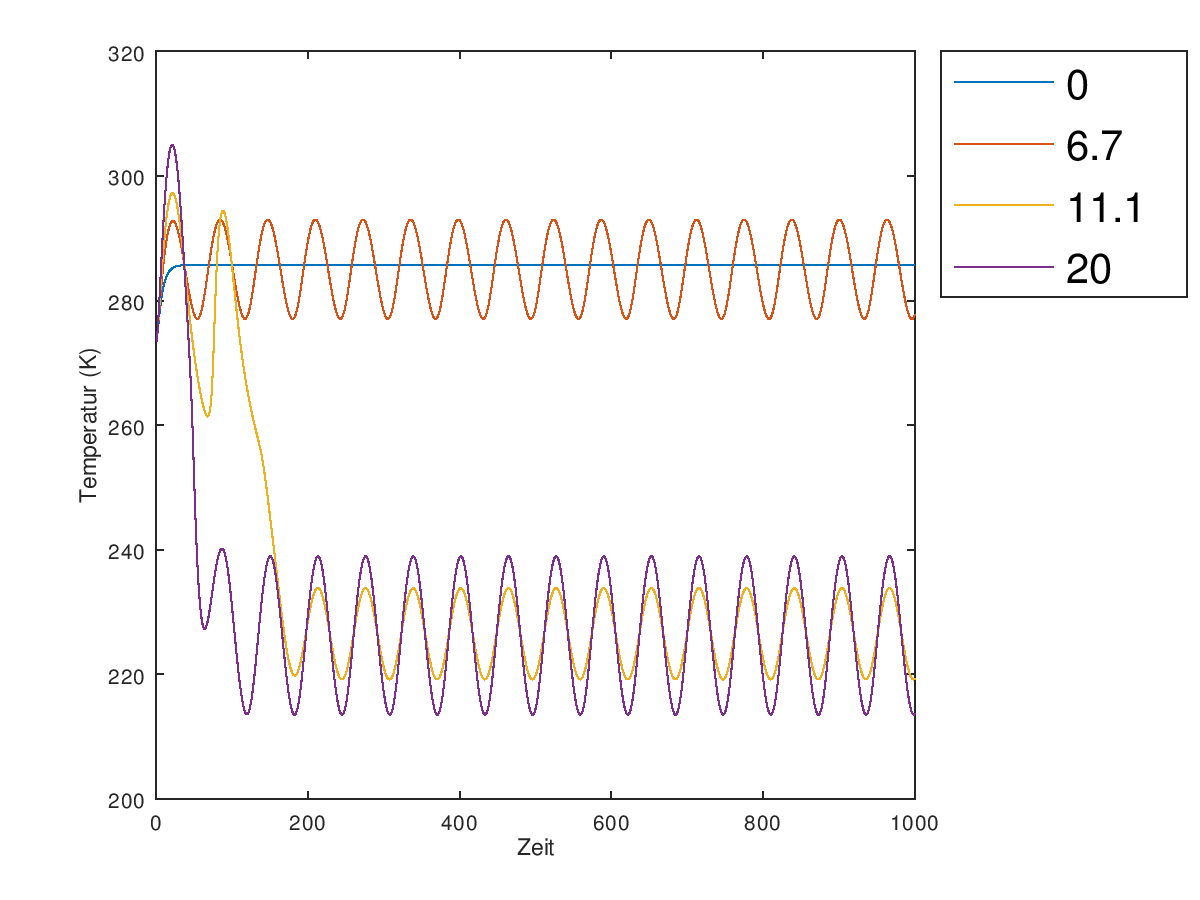
\includegraphics[width= 0.8\textwidth]{neigung/Zeitachse_3.png}
	\caption[Simulation II c]{Simulation II c}
	\label{fig:abb14}
\end{figure}
%

\section{Schlussfolgerung} \label{sec:schluss}
\rhead{Schlussfolgerung}
Die Neigung der Erdachse bewirkt die Jahreszeiten. Je stärker die
Erdachse geneigt ist, desto extremer Fallen diese aus. In dieser
Arbeit wurde gezeigt, wie dies mathematisch für eine Halbkugel
modelliert werden kann. Zudem wurde gezeigt, dass für die Erde zwei
Gleichgewichtstemperaturen bestehen. Durch einen extrem kalten
Winter kann es dazu kommen, dass die Erde von der warmen
Gleichgewichtstemperatur in die kalte Gleichgewichtstemperatur
wechselt. Dies würde zu einer Eiszeit führen. Um aus dieser Eiszeit
zu entkommen, wäre eine extreme Erwärmung der Erde notwendig, wie
sie möglicherweise durch Vulkanausbrüche stattfinden könnte.

Das mathematische Modell welches in dieser Arbeit verwendet wurde
fokussiert sich dabei auf eine Halbkugel. Es findet kein Energieaustausch
statt, die Jahreszeiten sind jeweils entgegengesetzt zwischen den
Erdhalbkugeln, womit es für die durchschnittliche Erdtemperatur nur
geringe Auswirkungen hat. Zudem ist die Ausstrahlung der Erde
weiterhin als schwarze Kugel modelliert.

Trotz dieser Vereinfachungen zeigt die Simulation wie es zu einer
Eiszeit kommen kann. Ein wichtiger Punkt dabei ist die Asymmetrie
der Coalbedo, wobei die Energieaufnahme der Erde bei tieferen
Temperaturen stärker reagiert als bei hohen Temperaturen. Ohne diese
Asymmetrie entscheidet sich die Art des Gleichgewichtes bereits in
der ersten Periode.

Es sei zum Schluss angemerkt, dass ein Zusammenspiel der Milankovi\'c
Zyklen dazu führen kann, dass ein kälterer Winter auftritt. Durch
die Exzentrizität kann es zu einer weiteren Distanz zwischen Erde
und Sonne kommen. Verbunden mit der Ekliptikschiefe, welche zu einem
höheren Neigungswinkel führt, kann somit eine Eiszeit entstehen.


\printbibliography[heading=subbibliography]
\end{refsection}
